\documentclass{article}
\usepackage{graphicx} % Required for inserting images
\usepackage{hyperref}
\usepackage{listings}
\usepackage{imakeidx}
\usepackage{float}
\makeindex
\title{Statistical Insights: Applying Inferential Analysis to Software Incident Data}
\author{
Milap Jhumkhawala \\
University of the Cumberlands
}

\date{October 2024}

\begin{document}


\maketitle
\newpage

\setcounter{tocdepth}{3} % Control depth of table of contents
\tableofcontents
\newpage

\section{Introduction}
 
In software development, it is essential to create release policies based on empirical evidence rather than speculation or tradition. There are often debates about the best practices for managing deployments, with differing opinions on how to mitigate risks effectively. Some argue for specific restrictions, such as limiting deployments on certain days or during particular time frames, while others advocate for more robust deployment processes. Enforcing arbitrary deployment restrictions without detailed analysis only masks the larger issues in the deployment process.

% A post on the AWS community titled \textit{“12 DevOps Best Practices That Make Deploying on Fridays Less Scary”} expands on this idea, emphasizing that the fear of Friday deployments often stems from poor DevOps practices. The article advocates for best practices like small batch deployments, trunk-based development, and feature flags to reduce risk, arguing that teams with well-automated and resilient processes should be able to deploy on any day without concern.

% , trend analysis, and evaluating the impact of deployments on incident frequency.

These differing opinions highlight a critical need for software teams to rely on data-driven policies for their release cycles. By applying inferential statistical analysis to incident data, teams can gain insights into when deployments pose the greatest risk. This white paper intends to perform various statistical analyses, including comparing incidents across days of the week and seasonal patterns. These analyses will provide actionable insights into reducing deployment risks and improving release strategies. By embracing data-driven policies, teams can develop more effective release policies designed to minimize incidents and outages.

\section{Key Concepts: Understanding Null Hypothesis Significance Testing (NHST)}
The social, behavioral, and biological sciences use NHST more frequently than any other inferential statistics technique at this time (Spatz, 2019). While learning about NHST (Null Hypothesis Significance Testing), I encountered an example, "Doritos states their nacho cheese flavor bag contains 269.3 grams of tortilla chips. How can we test this?" This made me think about whether a similar approach could be applied to analyzing assumptions or claims about incidents and the resulting release policies in software systems.

 
\subsection{Hypotheses Generation}
At its core, hypothesis testing is a statistical method used to evaluate assumptions or claims about a dataset (Spatz, 2019). The test typically begins by converting the claim or assumption into two competing hypotheses or logical possibilities.  

\subsubsection{Null Hypothesis ($H_0$)}

$H_0$ is a hypothesis of equality about parameters (Spatz, 2019). For example, $H_0$: Treatment A \textit{does not} have an effect; that is, the mean Q score (measure of potential risk of developing cardiovascular disease) of the population of those who received treatment A is equal to the mean Q score of the population of those who did not. Simply put, $H_0$ represents the logical possibility of NO difference between two groups.

\subsubsection{Alternative Hypothesis ($H_1$)}
$H_1$ is a hypothesis of the difference between two parameters (Spatz, 2019). For example, $H_1$: Treatment A \textit{does} have an effect; that is, the mean Q score (measure of potential risk of developing cardiovascular disease) of the population of those who received treatment A is \textit{not} equal to the mean Q score of the population of those who did not. Simply put, $H_1$ represents the logical possibility of SOME difference between two groups.

There are three possible alternative hypotheses, and the choice of an alternative hypothesis determines the conclusion of the analysis. 

\begin{itemize}

    \item Two-tailed test: 
    \begin{math}H_1: \mu_0 \neq \mu_1\end{math} The population parameters differ, but the order is not specified, making it inconclusive (could be lesser than or greater than)
    
    \item One-tailed tests:
        \subitem \begin{math}H_1 : \mu_1 < \mu_0\end{math} The population parameter less than that of $H_0$

        \subitem \begin{math}H_1 : \mu_1 > \mu_0\end{math} The population parameter greater than that $H_0$

\end{itemize}

\subsection{Significance Levels and p-values}

The result of hypothesis testing is evaluated using a p-value. In statistics, \textit{p} is the probability of the data obtained if the null hypothesis is true (Chang et al., 2019). Most analyses will report a p-value, and \textit{p} helps us determine whether to reject the null hypothesis or not.

\begin{itemize}
\item Low p-value (\begin{math} p < 0.05 \end{math}): There is strong evidence against the null hypothesis, meaning the result is statistically significant, and\textbf{ we reject the null hypothesis in favor of the alternative hypothesis}.

\item High p-value (\begin{math} p  \geq 0.05\end{math}): The observed data could easily occur under the null hypothesis, meaning the result is not statistically significant. We \textbf{fail to reject the null hypothesis}.

\end{itemize}

\subsection{Degrees of Freedom}

Degrees of Freedom or $df$ is a concept in statistics that refers to the number of independent values or quantities that can vary in a statistical calculation (Spatz, 2019). For example, if you are asked to pick two numbers and there are no restrictions, then both numbers are free to have any value; you have two degrees of freedom. In the context of t-tests, the general rule for calculating degrees of freedom is \textit{N} - 1 for one sample t-test and (\begin{math} n_1 + n_2 -2\end{math}) for Independent Samples t-test, where $n1$ is the sample size for Group 1 and $n_2$ is the sample size for Group 2


\section{Applying Hypothesis Testing}

With the foundational concepts of Null Hypothesis Significance Testing (NHST) established, we now transition to applying these principles to our software incident data.

\subsection{Dataset Source}

To conduct our analysis, we utilize the \href{https://www.kaggle.com/datasets/shamiulislamshifat/it-incident-log-dataset?resource=download}{IT Incident Log Dataset} from Kaggle. This dataset comprises event logs of an incident management process extracted from data gathered by the audit system of a ServiceNow™ platform instance used by an IT company. The event log is enriched with data loaded from a relational database underlying a corresponding process-aware information system. All information has been sanitized to protect privacy.

\subsection{Statistical Analysis Software JASP}

I will be utilizing \href{https://jasp-stats.org/}{JASP}, an open-source statistical analysis software, to perform various statistical tests on the incident data.

\subsection{Evaluating 'No Friday Deployments' Policy}

One widely debated topic is the practice of avoiding deployments on Fridays. A quick Google search of the question "Should you deploy on a Friday?" brings up a mix of articles—some strongly advising against it, while others support it but fail to provide clear explanations. 

Friday deployments are commonly avoided in the industry based on the belief that the risk of them causing outages or incidents is inherently high. (TODO talk about survey results, if any). 

% One of the main reasons cited by engineers and developers who participated in the survey was the possibility of a Friday deployment causing incidents over the weekend, requiring engineers to work during their time off. 
The fear is based on the assumption that Friday deployments are inherently riskier, leading to potential disruptions at inconvenient times. By subjecting the "no Friday deployments" belief to inferential statistical tests, we can move beyond this assumption and provide empirical evidence to either support or refute it. It wouldn't be entirely fair or accurate to state that the fear of Friday deployment is solely based on the assumption of inherent risk they carry. In reality, the fear could stem from many factors, such as cultural norms, past experiences, operational challenges, etc. However, based on my experience and research, the assumption that Friday deployments inherently carry more risk is a widely accepted belief. Ultimately, statistical analysis helps clarify whether Friday deployments are genuinely riskier based on data and whether it makes sense to establish release policies around this assumption.

Let's subject this belief to statistical hypothesis testing using the incident data from the dataset.

\subsubsection{Forming Hypotheses}

The first step is to convert the claim or belief into two competing hypotheses or logical possibilities.

\begin{itemize}
    \item Null Hypothesis ($H_0$): Friday deployments \textit{do not} lead to more incidents, OR There is no significant difference in the number of incidents on Fridays compared to other days of the week.

    \item Alternative Hypothesis ($H_1$): Friday deployments \textit{do lead} to more incidents, OR There is a significant difference in the number of incidents on Fridays compared to other days of the week
\end{itemize}

\subsubsection{Assumptions}

In this study, the following assumptions are made to guide the analysis:

\begin{itemize}
    \item Incident occurs on the same day as the Deployment.
    \item Friday deployment can lead to an incident on Friday
    \item Causality assumption that Deployments lead to Incidents
    \item No confounding variables, like a particular type of deployment, are more likely to happen on Fridays and are more likely to cause an incident.    
\end{itemize}


\subsubsection{Data Preparation}


The Kaggle dataset lacks a specific day-of-the-week attribute, which is essential for statistical tests. The following code snippet demonstrates the steps taken to generate this column using other existing columns in the dataset.

\begin{lstlisting}[language=Python, breaklines=true]
import pandas as pd
import os

data = pd.read_csv('it-incident-log-dataset/incident_event_log.csv')

\end{lstlisting}
\begin{lstlisting}[language=Python, breaklines=true]
# Add a column that formats the time the Incident was opened to a day of the week
\end{lstlisting}

\begin{lstlisting}[language=Python, breaklines=true]

data['opened_at'] = pd.to_datetime(data['opened_at'], format='%d/%m/%Y %H:%M', errors='coerce')
data[['opened_at']].head()    
\end{lstlisting}
\begin{table}[H]
\centering
\begin{flushleft}
\begin{tabular}{|l|}
\hline
\textbf{opened\_at} \\
\hline
2016-02-29 01:16:00 \\
2016-02-29 01:16:00 \\
2016-02-29 01:16:00 \\
2016-02-29 01:16:00 \\
2016-02-29 04:40:00 \\
\hline
\end{tabular}
\end{flushleft}
% \caption{Sample Output of the 'opened\_at' Column}
\end{table}

\begin{lstlisting}[language=Python]
data['day_of_week'] = data['opened_at'].dt.day_name()
data[['opened_at','day_of_week']].head()
\end{lstlisting}

\begin{table}[H]
\centering
\begin{flushleft}
\begin{tabular}{|l|l|}
\hline
\textbf{opened\_at} & \textbf{day\_of\_week} \\
\hline
2016-02-29 01:16:00 & Monday \\
2016-02-29 01:16:00 & Monday \\
2016-02-29 01:16:00 & Monday \\
2016-02-29 01:16:00 & Monday \\
2016-02-29 04:40:00 & Monday \\
\hline
\end{tabular}
\end{flushleft}
% \caption{Sample Output of the 'opened\_at' and 'day\_of\_week' Columns}
\end{table}
\begin{lstlisting}[language=Python, breaklines=true]
# Groups the dataset by month and day of the week, then counts the number of incidents for each combination, returning the result in a new DataFrame with an incident_count column. 
# Also, add a column called isFriday to indicate whether the incident occurred on a Friday.
\end{lstlisting}

\begin{lstlisting}[language=Python, breaklines=true]
incident_counts_per_day_month_all = data.groupby([data['opened_at'].dt.month, 'day_of_week']).size().reset_index(name='incident_count')
incident_counts_per_day_month_all['isFriday'] = (incident_counts_per_day_month_all['day_of_week'] == 'Friday').astype(int)
incident_counts_per_day_month_all
\end{lstlisting}

\begin{table}[htbp]
\centering
\begin{flushleft}
\begin{tabular}{|l|l|l|l|}
\hline
\textbf{opened\_at} & \textbf{day\_of\_week} & \textbf{incident\_count} & \textbf{isFriday} \\
\hline
1  & Friday    & 57  & 1 \\
1  & Monday    & 94  & 0 \\
1  & Saturday  & 14  & 0 \\

... & ...      & ... & ... \\
12 & Monday    & 49  & 0 \\
12 & Tuesday   & 25  & 0 \\
12 & Wednesday & 37  & 0 \\
\hline
\end{tabular}
\end{flushleft}
% \caption{Incident counts grouped by month, day of the week, and isFriday status}
\end{table}

\begin{lstlisting}[language=Python, breaklines=true]
# Export the data frame to csv as it is now ready to be used for performing statistical tests.
\end{lstlisting}


\begin{lstlisting}[language=Python, breaklines=true]
incident_counts_per_day_month_all.to_csv('incidents_counts_per_day_all_months.csv', encoding='utf-8', index=False)
\end{lstlisting}

\subsubsection{Load Data into JASP}

The first step is to load the data frame with the incident count per day of the week prepared in the previous section. Two columns are created:

\begin{figure}[H]
    \centering
    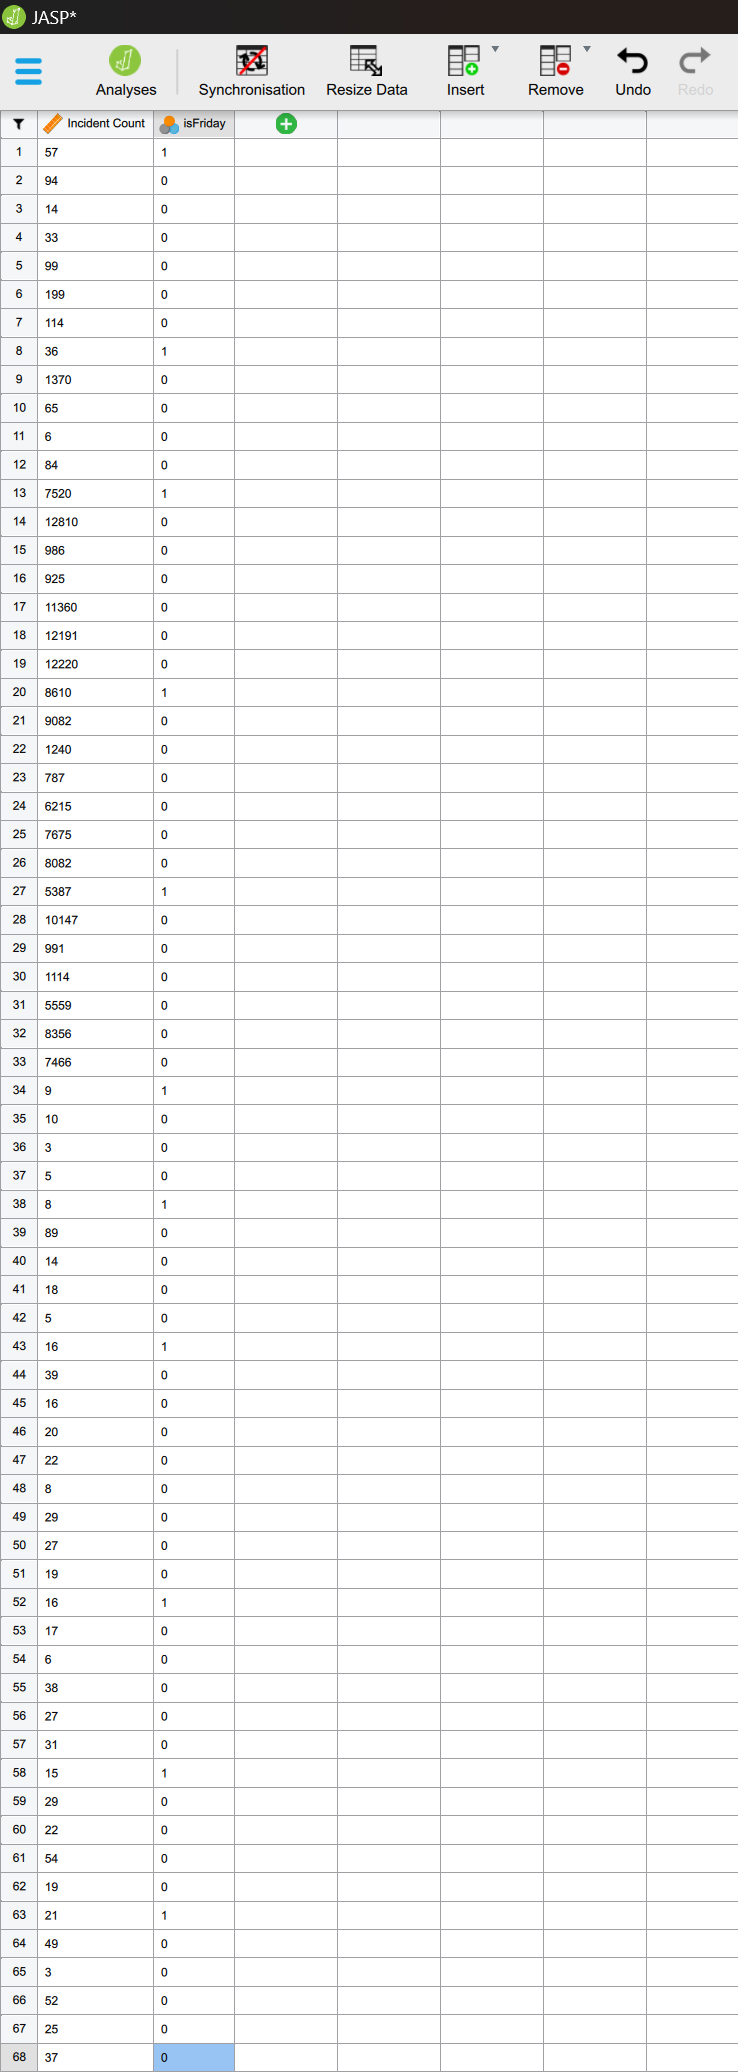
\includegraphics[width=0.5\linewidth, height=13cm]{Screenshot 2024-09-25 011255.png}
    \caption{Adding data to JASP}
    \label{fig:enter-label}
\end{figure}

\begin{itemize}
    \item Incident Count of Scalar data type
    \item isFriday of Nominal data type to represent categorical data, distinguishing incidents on Fridays from other days.
\end{itemize}


The second step is to choose the correct statistical test.

\subsubsection{Choosing Statistical Test}
To conduct Null Hypothesis Significance Testing (NHST) in this analysis, we need to apply a statistical test that will help us reject or not reject our null hypothesis. However, the type of Independent Samples T-Test to apply depends on assumptions like the probability distribution that the data is normal or whether variances(or spread) of two or more groups are equal. It is common practice to conduct preliminary tests to verify the assumptions before conducting other statistical analyses to avoid getting misleading or inaccurate results.

\begin{itemize}
    \item Shapiro-Wilk Test is used to measure if the data follows a normal distribution (Spatz, 2019). Based on the results of this test, we can decide whether to choose classical(parametric) or Mann-Whitney U (non-parametric) t-test

    \item Brown-Forsythe Test is used to measure the equality of variances of the two or more groups in the data (Spatz, 2019). Based on the results of this test, we can decide whether to choose classical or Welch's t-test
    
    We can let JASP handle this calculation for us.

    \begin{figure}[H]
        \centering
        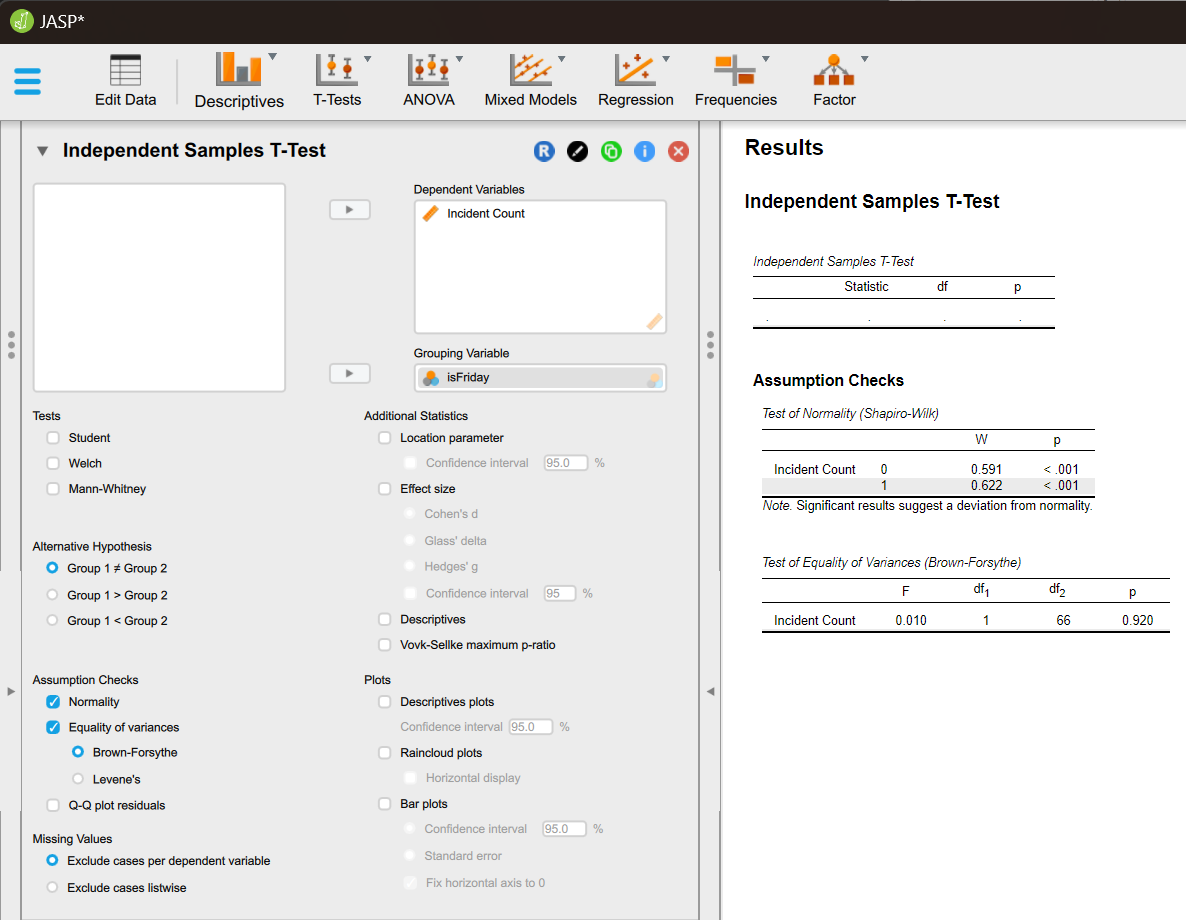
\includegraphics[width=0.7\linewidth, height=8cm]{Screenshot 2024-09-27 230725.png}
        \caption{Enter Caption}
        \label{fig:enter-label}
    \end{figure}

    Result Analysis:

    \begin{itemize}
        \item Test of Normality (Shapiro-Wilk): The p-values for both groups are less than 0.001, which is below the typical significance level of 0.05. This indicates that we reject the null hypothesis of normality, and we can conclude the data does not follow a normal distribution.

        \item Test of Equality of Variance (Brown-Forsythe): The p-value is 0.920, which is much greater than the significance level of 0.05. This means that we fail to reject the null hypothesis of equal variances. Thus, the assumption of equal variances holds true for this dataset.
    \end{itemize}

    Due to the violation of the normality assumption, it is appropriate to use a \textbf{non-parametric test} like the\textbf{ Mann-Whitney U test} instead of the classical or Welch's Independent Samples t-test.
    
\end{itemize}

\subsubsection{Mann-Whitney U Independent Samples T-Test}

This test is appropriate when comparing the means of two independent groups to determine if a statistically significant difference exists between them (Change et al., 2019). Specifically, in this case, we aim to determine whether the average number of incidents on Fridays is significantly greater than the number of incidents on other days. This method helps move beyond assumptions and offers empirical evidence to either support or refute the belief that Friday deployments lead to more incidents.

 However, it’s important to note that the conclusions drawn from this analysis are dependent on the specific dataset being used. The results may only reflect the patterns and trends present in this dataset and may not universally apply to all systems or organizations. Supporting or refuting the belief about Friday deployments will be tied to the characteristics of the incidents captured in this particular dataset.

 The test statistic is calculated using the formula:

 
\begin{equation}
U = \min \left( n_1 n_2 + \frac{n_1 (n_1 + 1)}{2} - R_1, \, n_1 n_2 + \frac{n_2 (n_2 + 1)}{2} - R_2 \right)
\end{equation}

Where:
\begin{itemize}
    \item $n_1$ = Sample size of group 1
    \item $n_2$ = Sample size of group 2
    \item $R_1$ = Sum of the ranks for group 1
    \item $R_2$ = Sum of the ranks for group 2
    \item $U$ = Mann-Whitney U statistic, which is the smaller of the two calculated \( U \)-values for the two groups
\end{itemize}

We can let JASP handle this calculation for us.

\begin{figure}[H]
    \centering
    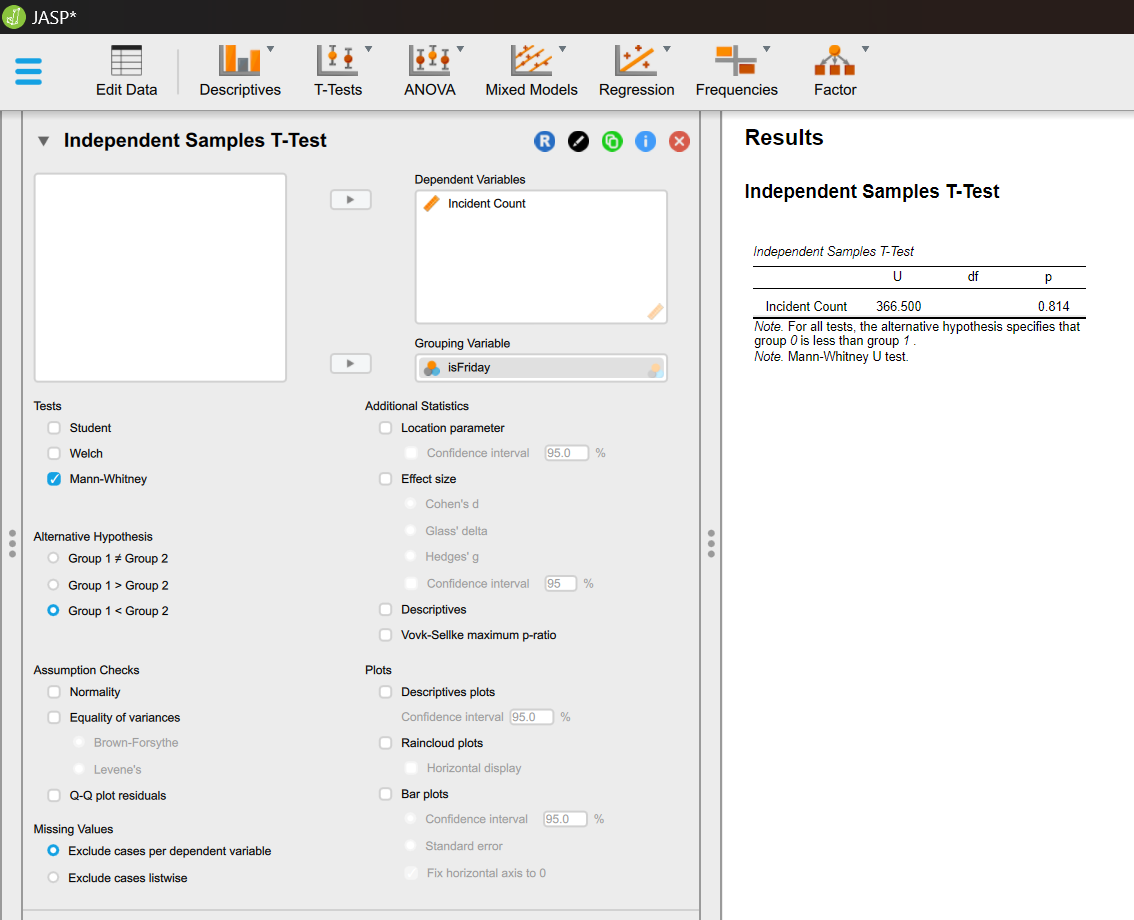
\includegraphics[width=0.7\linewidth]{Screenshot 2024-09-28 011601.png}
    \caption{Enter Caption}
    \label{fig:enter-label}
\end{figure}

\subsubsection{Result Analysis}

Since the p-value of 0.814 is much higher than 0.05, we \textbf{fail to reject the null hypothesis}. This suggests that there is no statistically significant evidence to indicate that incident counts on Fridays are higher than on other days of the week, challenging the belief that Friday deployments are inherently riskier based on this dataset. 

This type of statistical analysis can offer valuable data-driven insights that may not be immediately apparent. It also highlights the importance of developing or examining release policies based on empirical data and statistical evidence rather than relying on conventional traditions or assumptions.

\subsection{Seasonal Analysis}

The seasonal analysis aims to investigate whether incidents are more frequent during specific months, quarters, seasons, or holiday periods. In the software industry, it is common for organizations to implement a deployment freeze around certain holidays or peak seasons, prohibiting any new code deployments in production. While this might seem like a reasonable strategy from a high-level perspective, it is not always the best approach. For instance, certain periods like Black Friday or Christmas do experience higher user traffic, but establishing arbitrary code deployment deadlines introduces risks and can create additional problems once the freeze is lifted. Therefore, it is crucial not to enforce such policies without gathering empirical and statistical evidence to justify them.

Using the dataset, let's look at the heatmap below, which represents the incident density by month and week. 

\begin{figure}[H]
    \centering
    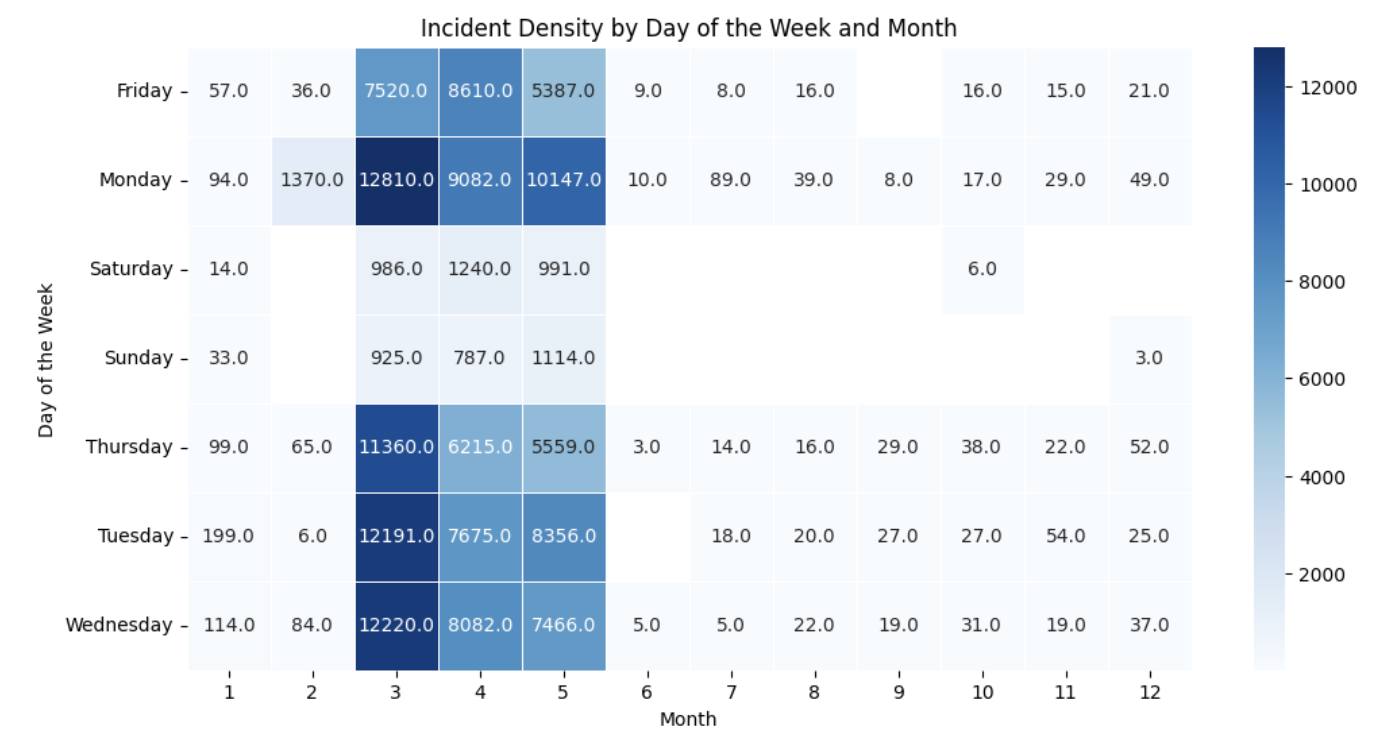
\includegraphics[width=0.7\linewidth]{Screenshot 2024-10-01 233549.png}
    \caption{Incident Density}
    \label{fig:enter-label}
\end{figure}

From the heatmap, we can observe a high density of incidents in March and April, particularly on Mondays, Tuesdays, and Wednesdays. I also want to highlight that an arbitrary \textit{No Friday Deployments} release policy might prove to be an ineffective strategy in this case. 

\subsubsection{Why Perform Statistical Inference Tests?}

Based on the heatmap, it is evident that incidents in March and April are significantly higher compared to other months, prompting the question: why is it necessary to perform further hypothesis testing when the trend appears so clear? While visual representations such as heatmaps are powerful tools for spotting trends and patterns, they can be deceptive without statistical validation. This is where the principle of scientific inquiry comes into play. Scientific inquiry demands that we move beyond subjective visual interpretations and apply rigorous mathematical testing to validate or refute our observations. Hypothesis testing, in this context, serves as a safeguard against jumping to conclusions based solely on visual cues.

\subsubsection{Forming Hypotheses}

The first step is to convert the question into two competing hypotheses or logical possibilities.
\begin{itemize}
    \item Null Hypothesis ($H_0$): There is no significant association between the month and the frequency of incidents. In other words, incident counts are uniformly distributed across all months, and any observed differences are due to random chance.

    \item Alternative Hypothesis ($H_1$): There is a significant association between the month and the frequency of incidents. In other words, at least one month has a significantly different number of incidents, indicating that the distribution of incidents varies by month.
\end{itemize}


\subsubsection{Data Preparation and Load Data into JASP}

\begin{lstlisting}[language=Python]
data['month'] = data['opened_at']
chi_sqaure_df = data.groupby('month')['incident_count'].sum().reset_index()
chi_sqaure_df.head()
\end{lstlisting}

\begin{table}[htbp]
\centering
\begin{flushleft}
\begin{tabular}{|l|l|}
\hline
\textbf{Month} & \textbf{Incident Count} \\
\hline
1 & 610 \\
2 & 1561 \\
3 & 58012 \\
4 & 41691 \\
5 & 39020 \\
\hline
\end{tabular}
\end{flushleft}
\label{tab:incident_count}
\end{table}

After this, we load this data frame into JASP, setting the Month column to type Nominal and Incident Frequency as Scale.

\subsubsection{Choosing Statistical Test}

Before Karl Pearson dreamed up the Chi-square, theory testers presented theoretical predictions and empirical data side by side, followed by a subjective judgment or conclusion about how well the theory matched the data, often labeled as \textit{good fit} or \textit{poor fit} (Spatz, 2019). However, with Chi Square, researchers could quantify the degree of "fit" and determine whether any differences between the predicted and observed values were due to chance or were statistically significant (Spatz, 2019). This moved hypothesis testing from subjective interpretation to a more rigorous, evidence-based practice.


When the data consists of categories and their frequency counts, the appropriate statistic to use for testing relationships between these categories is the Chi-Square test. The Chi-Square test is designed to compare observed frequencies (the number of occurrences in each category) with expected frequencies (what we would expect if there were no significant relationship or association between the categories) (Spatz, 2019). This test is particularly useful for categorical data, where the focus is on how often certain events or categories occur.

For example, suppose we have data on the number of incidents that occur in different months, and we want to test whether incidents are uniformly distributed across all months. In that case, the Chi-Square test allows us to see if the observed frequencies (incident counts for each month) significantly deviate from the expected frequencies (if the incidents were distributed evenly across months). This is especially relevant when we want to understand whether specific months have more incidents than would be expected by chance.

\subsubsection{Chi Square Test}

% Hypothesis: Are incidents more frequent in certain months or seasons?
% Test: Perform a chi-squared test or ANOVA to analyze the distribution of incidents across different seasons or quarters.
% Null Hypothesis (H0): There is no significant difference in incident counts across different months or seasons.
% Alternative Hypothesis (H1): There is a significant difference in incident counts across months or seasons.

The Chi-Square test is used to determine if there is a significant association between categorical variables. In this context, the test evaluates whether the distribution of incidents varies significantly across different months or seasons. The Chi-Square test is particularly useful when dealing with frequency data and helps verify whether any observed differences are due to random chance or reflect a meaningful pattern.

\begin{equation}
\chi^2 =  \sum \frac{(O_i - E_i)^2}{E_i}
\end{equation}

Where:
\begin{itemize}
    \item $O_i$ = Observed frequency for category \textit{i} or actual count of incidents
    \item $E_i$ = Expected frequency for category \textit{i} or the expected count of incidents in each month if they followed some expected pattern. In a test for equal proportions, the expected frequency would be the total number of incidents divided equally among all months.
    \item $\chi^2$ = Chi-Square statistic
\end{itemize}

We can let JASP calculate the Chi-Square statistic and give us the p-value.

\begin{figure} [H]
    \centering
    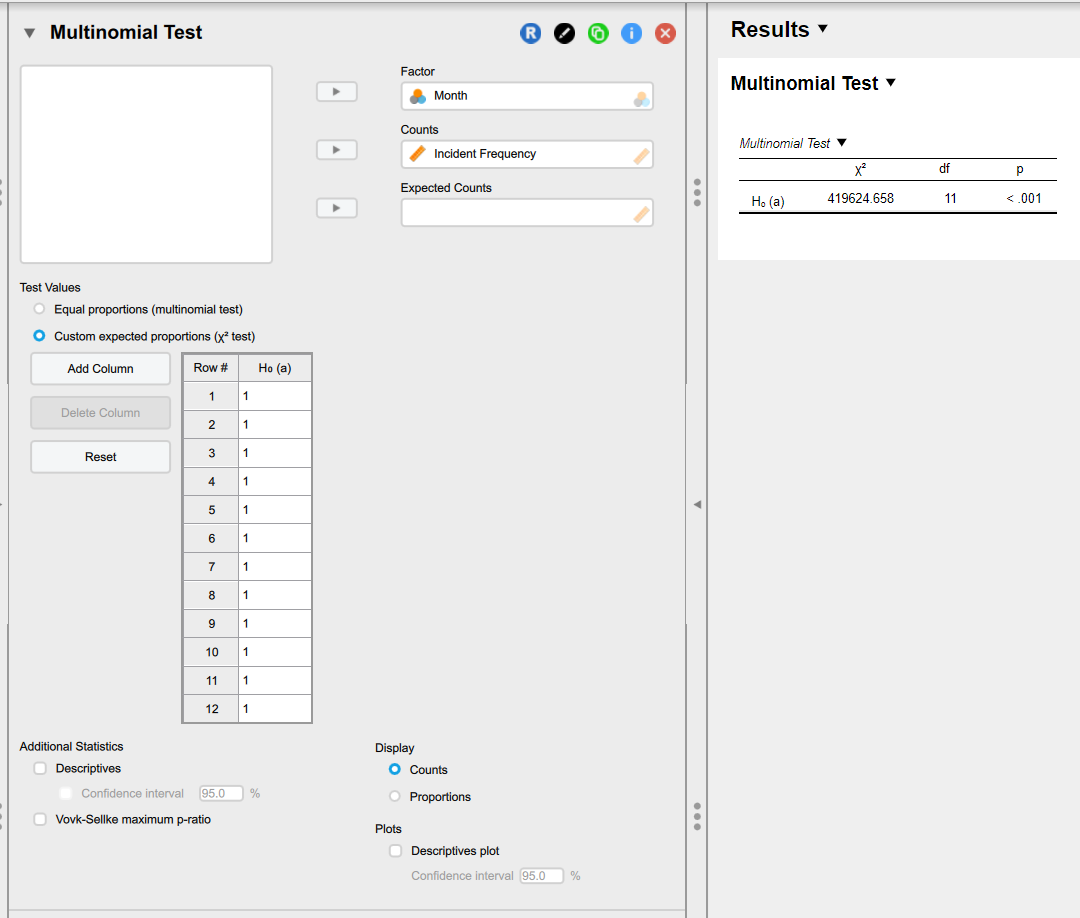
\includegraphics[width=0.5\linewidth]{Screenshot 2024-10-20 170522.png}
    \caption{Chi-Square Test}
    \label{fig:enter-label}
\end{figure}

\subsubsection{Result Analysis}

Since the p-value is $< 0.01$, which is much lesser than 0.05, \textbf{we reject the null hypothesis}, this result supports the Alternative Hypothesis($H_1$), indicating that some months (particularly March and April, based on our observed data) have a significantly higher number of incidents compared to others. The large variation in incident counts between months suggests that factors such as seasonal patterns or specific operational conditions might be influencing the frequency of incidents. Therefore, monthly patterns should be taken into account when analyzing incident trends and making decisions about release or deployment strategies.

\section{Conclusion}

In conclusion, this white paper has demonstrated the importance of using empirical evidence, such as statistical analysis, to inform release policy decisions in software development. Through various statistical tests that were carefully chosen, we analyzed the incident data to challenge arbitrary release policies observed in the industry, which may lead to inefficiencies and unnecessary risk. Instead, data-driven insights offer a more reliable foundation for making informed decisions, ensuring that release strategies are optimized for the actual patterns of incidents, ultimately leading to more resilient software systems.


\newpage

\section{References}

Spatz, C. (2019). Exploring statistics: Tales of distributions. (12th ed.). Conway, AR: Outcrop Publishers. 

\vspace{5mm}

\noindent Chang, M., Balser, J., Roach, J., \& Bliss, R. (2019). Innovative strategies, statistical solutions and
simulations for modern clinical trials. CRC Press, Taylor \& Francis Group.

\end{document}

